\subsection{Algebra and calculus background}

\ssn{Combinations}
 \begin{itemize}
 \item The number of ways of choosing $k$ things from $n$ with order taken into consideration is 
  \[       \frac{n!}{(n-k)!}.
   \]
  \item 
    The number of ways of choosing $k$ things from $n$ with order NOT taken into consideration is the \emph{binomial coefficient} 
  \[     \binom{n}{k} =  C^n_r = \frac{n!}{k!(n-k)!}.
   \]
 \end{itemize}
\end{n}

\ssn{Calculus}
  \begin{itemize}
    \item   $\int_{-\infty}^\infty e^{-x^2} \dd x = \sqrt{\pi}$
  \end{itemize}
\end{n}

\ssn{Stirlings formula and Gamma functions}
\begin{itemize}
\item For large $n$ we have Stirling's approximation
 \[
     n! \approx \left( \frac ne \right)^n \sqrt{2\pi n}. 
 \]
\item The gamma function is defined for real $x>0$ by 
 \[
   \Gamma(x) = \int_0^\infty u^{x-1}  e^{-x} \dd x.
 \]
Integration by parts shows that 
 \[
     \Gamma(x+1) = x \Gamma x. 
 \]
For natural numbers $n$, $\Gamma(n) = (n-1)!$. 
\end{itemize}

\end{n}


\section{Extras - to be incorporated} 

\ssn{Sample spaces and events}
The \emph{sample space} $S$ of an experiment is the set of all possible outcomes. An \emph{event} is a subset of the sample space. 

Given two events $A, B$ we can consider the union $A \cup B$ which is the event that at least one of $A$ and $B$ occur. We can also consider the intersection $A \cap B$ which is the event that both $A$ and $B$ occur. If $A \cap B = \{\}$ then $A$ and $B$ have no outcomes in common and so $A$ and $B$ can never occur together. We say that $A$ and $B$ are \emph{exclusive}.   

We write $A^c$ for the \emph{complement} of $A$. The complement of $A$ is the event which occurs precisely when $A$ does not occur.   
\end{n}

\ssn{Probability functions} 
A probability function assigns to each event $A \subseteq S$ a probability $\PP(A)$ in such a way that the following hold.  
\begin{enumerate}
\item $\PP(S) = 1$.
\item If $A$ is an event then $0 \leq \PP(A) \leq 1$. 
\item If $ A \subseteq B$ then $\PP(A) \leq \PP(B)$.
\item If $A \cap B = \{ \}$ then $\PP(A \cup B) = \PP(A) + \PP(B)$. 
\end{enumerate}
Note that because $A \cup A^c = S$ and $A \cap A^c = \{ \}$ the above imply that $\PP(A) + \PP(A^c) = 1$ and hence that $\PP(A^c) = 1-\PP(A)$.  

In the examples we have been considering, an event $A$ has consisted of a finite number of outcomes: $A= \{ a_1, \dots, a_k\}$. In that case, $\PP(A) = \PP(a_1) + \dots + \PP(a_k)$ and the properties above are obvious\footnote{Since probability functions are meant to apply to have arguments that are subsets of $S$ rather than individual elements, we should really write $\PP(\{ a_1\})$. We will however be lax on this point.}.   
\end{n}

\ssn{Geometric random variables} \label{geom_dist}
I roll a 6-sided die and let $X$ be the number of rolls until I roll a 6. What is the expected value of $X$?   Actually let us be more general and ask in general what is the expected number of tries before I have a ``success'', where independently on each roll I succeed with probability $p$ (where $0<p<1$) and fail with probability $1-p$.  So we have a random variable whose possible outcomes are $x_1=1,x_2=2,\dots, x_k = k, \dots$. 

We can compute $p_k$ using a tree: for $X=k$ we have to fail $k-1$ times (probability $1-p$ each time) and then succeed on the $k$-th attempt (probability $p$).   Thus we have 
\[
  p_k = (1-p)^{k-1} p, \quad \EE(X) = \sum_{k=1}^\infty k (1-p)^{k-1} p. 
\]
To evaluate the sum, write out $\EE(X)$ and $(1-p)\EE(X)$ as follows. 
 \begin{eqnarray*}
 \EE(X) & =&  p + 2(1-p)p + 3(1-p)^2p + 4(1-p)^3p + \dots \\
 (1-p)\EE(X) & = &  \phantom{ p + 2}(1-p) p + 2(1-p)^2p + 3(1-p)^3p  + \dots . 
 \end{eqnarray*}
Now subtract and cancel a $p$ from each side to deduce that
 \[
   \EE(X) = 1 + (1-p) + (1-p)^2 + (1-p)^3 + \dots =  \frac{1}{p}, 
 \]
 where for the last equality one sums a geometric series. 
We will see this again, and also other examples of ``standard random variables'' as we proceed. 

So the answer to our original dice question is that the expected number of rolls until we roll a 6 is six.  You might say this is not surprising, but it is not clear that it \emph{has} to be that way. 
\end{n}

\ssn{problem from twitter} 
Roll a D6 repeatedly until one gets a 6.  Suppose the six occurs on the $N$-th roll. Then we know that the expected value of $N$ is 6 by several arguments. 

What is the expected value of $N$, if you condition on there having been no odd numbers rolled before the first 6?   It may be a little unclear what this means.   For clarity then say it like this. Generate a number $x$ as follows. Roll a D6 until until you get a 6 and count the number of rolls, BUT additionally abandon your attempt and start over again if at any point you roll an odd number before you get your 6. What is the expected value of $x$? 

\paragraph{First approach} 
First forget about the odd number condition. Let  
 \[
  S = \{ \text{sequences of die rolls terminating at the first 6} \}
  \]
be the sample space. To a sequence of length $n$ attach the probability $1/6^n$.  Let $X$ be the rv that is the length of a given sequence. Then there are $5^{n-1}$ sequences of length $n$ and so 
 \[
            \EE(X) = \sum_{n=1}^\infty \frac{5^{n-1}}{6^n} = 6. 
  \]
Consider the subset $T\subseteq S$ consisting of al sequences with no odd entries. Then there are $2^{n-1}$ such sequences of length $n$ in $T$ and so 
  \[
     \PP(T) = \sum_{n=1}^\infty \frac{2^{n-1}}{6^n} = \frac{1}{4}. 
   \]
Thus, $\PP(X=n \st T) = 4\, \PP(\text{$X=n$ and $T$})$.   So 
 \[
   \EE(X \st T ) = \sum_{n=1}^\infty n\, \PP(X=n \st T) = 
   \sum_{n=1}^\infty 4n \,\PP(\text{$X=n$ and $T$}) = 
    \sum_{n=1}^\infty 4n \, \frac{2^{n-1}}{6^n} = \frac32. 
 \]

\paragraph{Second approach}
Consider that dice rolling procedure to generate a single sample from $X$ conditioned on $T$.  Let us say that when we start, the probability of getting an odd number before a 6 and having to start counting again is $w$. Conditioning on the first step, if one rolls an odd number then we certainly have to start again, if we roll a 6 we certainly do not, and if we roll a 2 or 4, the probability remains at $w$. So
\[
     w = \frac16 0 + \frac36 1 + \frac26 w 
\]
and solving, $w=3/4$. 

Now compute the expectation $g$ by conditioning on the first step. If we roll a 6 the expectation is 1. If we roll 1,3 or 5 we start again and so the expectation is $g$.   If we roll a 2 or 4 then from above the probability of having to abandon and start again is $3/4$ and otherwise the expected value is $g+1$. So 
 \[
     g = \frac16 1 + \frac36 g + \frac26 \left(  \frac34 g + \frac14 (g+1)       \right) 
 \]
 which is trivially solved to get $g=3/2$. 



\end{n}


\subsection{Grading}
This course will use a form of ``specifications grading'' for hand-ins and exams where individual items are judged against a rubric rather than a conventional mark scheme. 
\begin{table}[p] 
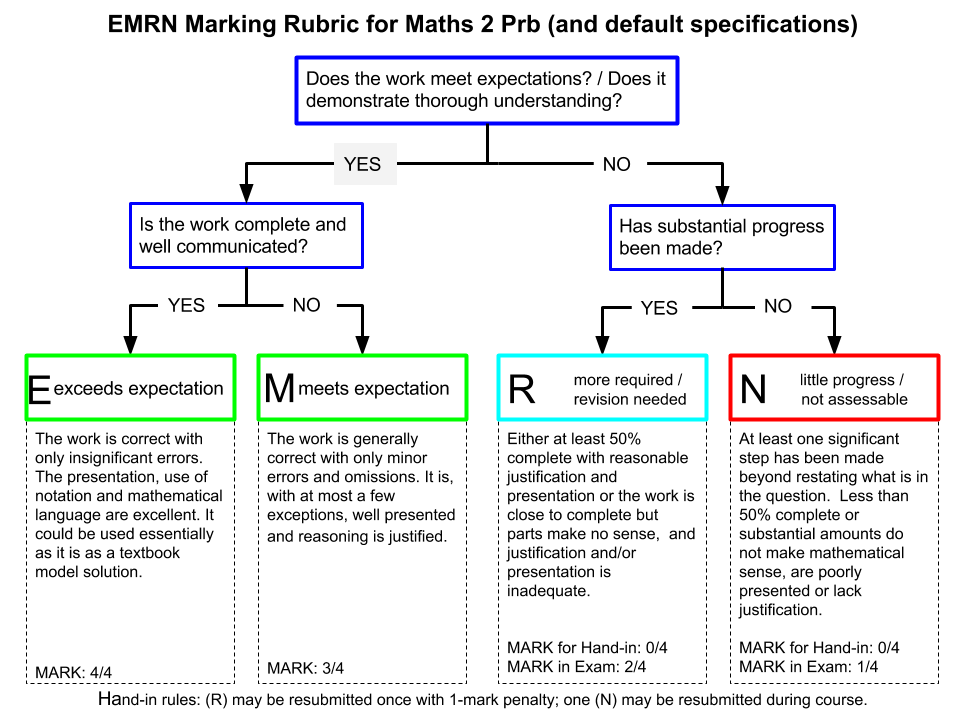
\includegraphics[width=21cm,angle=270]{images/EMRN_Rubric.png}
\end{table}

\section{Problems}

\ssp 
Your friend rolls two D6 and keeps them hidden from you. You ask your friend, ``is there at least one six?'' and he replies ``yes''.  What is the probability that he has rolled a double? 
\end{e} 

\sss
The probability is $1/11$. This is because there are exactly 11 equally likely possible rolls containing at least one six, but only one of them is a double. 
\end{s}

Yah-Tze Same problem and rules, but now the aim is throw five D6 until all are showing the same?  (Challenge --- be careful of an ``edge case''!)


\ssn{Definitions and notation}
An \emph{event} in probability is something that either does or does not happen. The mathematical way this is expressed is that we identify an event with the subspace of the sample space where it happens. 

So, for example, if we toss a coin 3 times a possible event is that we obtain precisely one H.  This event is identified with the subspace 
 \[
 A=\{ TTH, THT, HTT \} \subseteq \{ TTT, TTH, THT, THH, HTT, HTH, HHT, HHH \}. 
 \]
 
If we have another event $B$ defined to be ``the first coin is a T'' then we can consider the event that both $A$ and $B$ happen. This event is denoted $A \cap B$ since it corresponds to the intersection of the two sets. In this case, 
 \[
     A \cap B = \{ TTH, THT \} . 
 \]
\end{n}

\ssn{Definition}
Let $A$ and $B$ be events. We say that $A$ and $B$ are \emph{independent} if  
\[
     \PP( A \cap B ) = \PP(A) \PP(B). 
 \]
\end{n}

\ssn{Examples}
\begin{enumerate}
\item Roll two D6 and let $A$ be the event that the first roll is a `6' and $B$ be the event that the second roll is a `6'.  Then ``$A\cap B$'' is the event of rolling double 6.    We know $\PP(A) = \PP(B) = 1/6$ and also that $\PP(\text{double 6}) = 1/36$.  So $A$ and $B$ are independent.
\item Consider the example of tossing 3 coins as just above. We have $\PP(A) = 3/8$ since it corresponds to 3 of the 8 equally likely outcomes. Also $B = 1/2$.   As we observed, $A \cap B$ corresponds to two outcomes and so $\PP(A \cap B) = 1/4$. We see that $A$ and $B$ are not independent. 
Intuitively, this is because \emph{knowing the first coin is a T changes the probability of there being one H overall (from $3/8$ to $1/2$); one even is affecting the outcome of the other.}
\end{enumerate}
\end{n}

Generalise this formula to the case where $X$ has a Binomial distribution with parameters $n,p$ and $k=np$ is an integer.  Find an approximate formula for $\PP(X=k)$ when $b=n$ is large.  



\ssn{Sample spaces and events}
As we have seen, a \emph{sample space} $S$ is the set of all possible outcomes of an experiment or process. We identify some subsets of $S$ as being \emph{events}, which will be the things that have probabilities associated with them. We require the collection of vents to have the following properties. 
\begin{enumerate}[S1]
\item The whole sample space $S$ and the empty set $\emptyset$ are events. 
\item If $A \subseteq S$ is an event then $A^c = S \setminus A$ is also an event. (It is the event that happens precisely when $A$ does not happen.)
\item Secondly, if $A_1,A_2, \dots$ is a finite or countable collection of events then $\bigcup_i A_i$ is an event. It corresponds to at least one of the $A_i$ happening. 
\end{enumerate}
Events are going to be the occurrences to which we can associate probabilities.  In all the examples we have considered previously, every subset of $S$ is an event. But we will see later that for continuous distributions this is not the case. 
\end{n}

Take three D6 and roll them until you have a triple (i.e.\ all faces show the same number) when you stop. The rules are as follows. On the first round, roll all three. On the second round, you can keep any number of the dice and roll the rest. (So if you have two showing the same, you keep those and roll the third.) Continue for as many rounds as it takes to get the triple.  What are the probabilities of succeeding on (a) the first round; (b) the second round and (c) the third round?  (Give exact answers, and also evaluate these as a decimal.)

\ssn{Sampling with and without replacement}
I roll a D6 twice. What is the probability that I get a `1' followed by a `6'? Answer: $(1/6) \times (1/6) = 1/36$. 

I have a pack of 10 cards numbered 1 to 10. I choose one at random and then \emph{without replacing it} choose another from the pack.  (a) What is the probability that the first card is the `1'?  (b) What is the probability that the second card is the `10'.   (c) What is the probability that I get the `1' followed by the `10'? 

The answers to (a) and to (b) are both $1/10$.  To calculate the answer to (c) consider taking the first card: clearly the probability of its being `1' is $1/10$. Now however there are only 9 cards left and so \emph{knowing that the first card was a `1'} the probability of getting a `10' with the second draw is $1/9$. Therfore the answer (draw a tree if you need to) is $(1/10) \times (1/9) = 1/90$.   

Drawing a `1' first time has made it a little more likely that we draw a `10' next. \emph{The two events are not independent.} 

In terms of conditional probabilities we are reasoning as follows. 
\[
 \PP(\text{`1' then `10'}) = \PP(\text{first is `1'})   
 \, \PP( \text{second is `10'} \st \text{first is `1'}). 
\]

Finally, in more abstract language, let $A$ be the even that the first draw is the `1' and let $B$ denote the event that the second draw is the `10'. Then 
 \[
 \PP( A \cap B ) = \PP(A)\, \PP(A \st B) = \frac{1}{10} \, \frac19 = \frac1{90}. 
 \]
\end{n}

As a first example, suppose we roll two D6.  What is the probability that there is at least one `6' showing?   To solve this, let $A_1$ be the event that the first die shows a `6' and let $A_2$ be the event that the second die shows a `6'.  Clearly $\PP(A_1) = \PP(A_2) = 1/6$. The event $A_1 \cap A_2$ is rolling `double-6' and so $\PP(A_1 \cap A_2) = 1/36$. The event we are interested in is $A_1 \cup A_2$ and by the formula 
 \[
    \PP(A_1 \cup A_2) = \frac16 + \frac16 - \frac1{36} = \frac{11}{36}. 
 \]
 We computed this also by a simple table or tree previously. 
 
 
 \ssn{Definition} 
Let $A,B$ be events with $\PP(B) \not=0$. Then the \emph{conditional probability of $A$ given $B$} is defined by 
 \[
    \PP(A \st B) = \frac{ \PP( A \cap B)}{\PP(B)}. 
 \]
\end{n}

\ssn{Comments}
The conditional probability $\PP (A \st B)$ is the probability of $A$ occurring if we already know that $B$ has occurred.  

We have used conditional probabilities before, particularly in tree calculations.  Generally we were using the alternative form 
\[
    \PP(A\cap B) = \PP(A \st B) \PP(B) . 
\]
\end{n}

\begin{figure}
\begin{minipage}{0.47\textwidth}
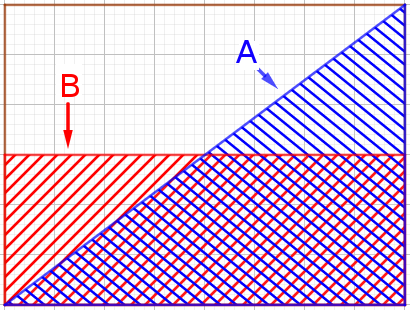
\includegraphics[width=0.95\textwidth]{images/conprob2.png} 
\end{minipage}%
\begin{minipage}{0.47\textwidth}
Imagining probabilities as being proportional to area, $\PP(A)=\PP(B) = 1/2$ and $\PP(A \cap B)=3/8$ (see picture on left). Thus $\PP(A \st B) = 3/4$. 

\hspace*{2ex}
If we ``zoom in on $B$'' as below we see that $A$ occupies three quarters of $B$. 

\vspace*{2ex}
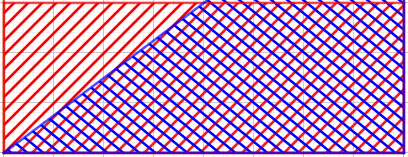
\includegraphics[width=0.95\textwidth]{images/conprob2r.png}
\end{minipage}
\caption{Conditional probabilities, imagining probability proportional to area}
\end{figure}

\ssn{Proposition}
\begin{itemize}
\item If $\PP(B) \not=0$ then $A,B$ are independent if and only if $\PP(A \st B) = \PP(A)$.
\item If $\PP(A) \not=0$ then $A,B$ are independent if and only if $\PP(B \st A) = \PP(B)$.  
(The proof is immediate from the definition.) 
\end{itemize}
\end{n}

\ssp 
We will solve a problem that caused some consternation recently on twitter. We know that the expected number of rolls of a D6 until we get a `6' is $6$. The question asked was this: what is the expected number of rolls until we get a `6', conditioned on the whole sequence consisting of even numbers? 
\begin{enumerate}
\item What do you imagine the answer might be, if you had to guess?
\item Describe how you would do an experiment to try and answer the question numerically. 
\item I give you a D6 and ask you to do some experiments to find this expected value.  What should you do? 
\item Take as sample space $S$ the set of all sequences of rolls of a D6, terminating with the first occurrence of a `6'.  What is the probability of a particular sequence of length $k$?  How many such sequences are there?  (This should fit with the formula for a geometric distribution.) 
\item You roll a D6 until you get a `6'. What is the probability that you have rolled no odd numbers in the process.  (You will need to 
\end{enumerate}

\end{e}



\ssn{Another tree example} 
An ``$n$-sided die'' is a real or imaginary object that chooses an element of $\{ 1,2,\dots, n \}$ uniformly randomly.  We will call such a thing a ``D$n$''. You can buy a D$n$ for many values of $n$ in gaming shops. 

Player A rolls a D3 and player B rolls a D4 and the winner is the person who rolls the higher number. In this rather unfair game, what are the probabilities that player A wins, draws and loses?   We will draw a tree, imagining that A rolls first. We will write $a$ for A's roll. Note how the labels on the arrows emerging from a node add up to $1$.  

\tikzset{
  treenode/.style = {shape=rectangle, rounded corners,
                     draw, align=center,
                     top color=white, bottom color=blue!20},
  root/.style     = {treenode, font=\Large, bottom color=red!30},
  env/.style      = {treenode},
  branch/.style = {treenode, bottom color=blue!10},  
  dummy/.style    = {circle,draw}
}
\tikzstyle{level 1}=[level distance=3.0cm, sibling distance=4.5cm]
\tikzstyle{level 2}=[level distance=8.5cm, sibling distance=1.5cm]
\begin{tikzpicture}
  [
    grow                    = right,
    edge from parent/.style = {draw, -latex},
    every node/.style       = {font=\normalsize}
  ]
\node[root]{Start}
child {
    node[branch]{$a=1$}
    child {
        node[env]{A win $(p=\frac{0}{12})$}
        edge from parent node[above,pos=0.7] {$0$}
        }
        child {
        node[env]{draw~~$(p=\frac{1}{12})$}
        edge from parent 
        node[above,pos=0.7] {$\frac{1}{4}$}
        }
       child {
        node[env]{B win $(p=\frac{3}{12})$}
        edge from parent 
        node[above,pos=0.7] {$\frac{3}{4}$}
        }  
    edge from parent 
    node[above] {$\frac{1}{3}$}
    }
    child {
    node[branch]{$a=2$}
    child {
        node[env]{A win  $(p=\frac{1}{12})$}
        edge from parent 
        node[above,pos=0.7] {$\frac{1}{4}$}
        }
        child {
        node[env]{draw~~$(p=\frac{1}{12})$}
        edge from parent 
        node[above,pos=0.7] {$\frac{1}{4}$}
        }    
        child {
        node[env]{B win $(p=\frac{2}{12})$}
        edge from parent 
        node[above,pos=0.7] {$\frac{2}{4}$}
        }    
    edge from parent 
    node[above] {$\frac{1}{3}$}
    }
    child {
    node[branch]{$a=3$}
    child {
        node[env]{A win $(p=\frac{2}{12})$}
        edge from parent 
        node[above,pos=0.7] {$\frac{2}{4}$}
        }
        child {
        node[env]{draw~~$(p=\frac{1}{12})$}
        edge from parent 
        node[above,pos=0.7] {$\frac{1}{4}$}
        }   
        child {
        node[env]{B win $(p=\frac{1}{12})$}
        edge from parent 
        node[above,pos=0.7] {$\frac{1}{4}$}
        }   
    edge from parent 
    node[above] {$\frac{1}{3}$}
    };           
\end{tikzpicture}


You should check all the calculations. As an example, near the top there is an edge labelled ``$2/4$'' that leads to a win for A.  What that means is that \emph{if we know that A has rolled a 3}, then the probability that A wins is $2/4 = 1/2$. This is true because when $a=3$, A wins if B rolls a 1 or 2 but draws or loses if B rolls 3 or 4. 
\end{n}



\ssn{A diversion (optional)}
I have a floor ruled with parallel lines unit distance apart. I take some stiff, thin wire of length $L$ and bend it into a reasonably smooth curve of some sort that will lie flat on the plane.  I toss the wire in the air so that it lands randomly on the floor.  What is the expected number of times the curved wire meets the ruled lines? 

You could approximate the the wire by a large number $n$ of straight line segments of length $L/n$. Let $X_j$ be the random variable that is $1$ if the $j$-th segment crosses a line and zero otherwise. Then 
 \[
    X = X_1 + X_2 + \dots + X_n 
 \]
 where $X$ is the total number of times the curve meets the lines. 
 
 Then the expected number of crossings of the whole curve in this approximation is given by 
 \[
 \EE(X) =  \EE\left(  \sum_{j=1}^n X_j \right) =  \sum_{j=1}^n \EE(X_j).
  \]
Now, $\EE(X_j)$ must be independent of $j$: it is the expected number of crossings of the lines on the floor by a randomly tossed line segment of length $L/n$.  The conclusion of all this is that the expected number of crossings must be proportional to $L$.  

Now a circular piece of wire of length $\pi$ has diameter $1$ and however it lands, it must meet the lines twice. So that fixes the constant of proportionality:
\[
      \EE(X) = \frac2\pi L 
\]

An interesting special case is to consider a straight line segment of unit length. In that case (neglecting a probability zero possibility of its (just) meeting two lines), $X$ takes only the values $0$ and $1$. Because of that, $\EE(X) = \PP(X=1)$. So the conclusion is that if you drop a unit length line segment randomly onto parallel lines unit distance apart, there is a probability of $2/\pi$ that it will cross a line. 
\end{n}
